\documentclass[letterpaper,final,12pt,reqno]{amsart}

\usepackage[total={6.3in,9.2in},top=1.1in,left=1.1in]{geometry}

\usepackage{times,bm,bbm,empheq,fancyvrb,graphicx}
\usepackage[dvipsnames]{xcolor}
\usepackage{longtable}

\usepackage{tikz}
\usetikzlibrary{decorations.pathreplacing}

\usepackage[kw]{pseudo}
\pseudoset{left-margin=15mm,topsep=5mm,idfont=\texttt}

% hyperref should be the last package we load
\usepackage[pdftex,
colorlinks=true,
plainpages=false, % only if colorlinks=true
linkcolor=blue,   % ...
citecolor=Red,    % ...
urlcolor=black    % ...
]{hyperref}

\renewcommand{\baselinestretch}{1.05}

\newtheorem{lemma}{Lemma}

\newcommand{\Matlab}{\textsc{Matlab}\xspace}
\newcommand{\eps}{\epsilon}
\newcommand{\RR}{\mathbb{R}}

\newcommand{\grad}{\nabla}
\newcommand{\Div}{\nabla\cdot}
\newcommand{\trace}{\operatorname{tr}}

\newcommand{\hbn}{\hat{\mathbf{n}}}

\newcommand{\bb}{\mathbf{b}}
\newcommand{\bbf}{\mathbf{f}}
\newcommand{\bg}{\mathbf{g}}
\newcommand{\bn}{\mathbf{n}}
\newcommand{\bu}{\mathbf{u}}
\newcommand{\bv}{\mathbf{v}}
\newcommand{\bw}{\mathbf{w}}
\newcommand{\bx}{\mathbf{x}}

\newcommand{\bV}{\mathbf{V}}
\newcommand{\bX}{\mathbf{X}}

\newcommand{\bxi}{\bm{\xi}}

\newcommand{\bzero}{\bm{0}}

\newcommand{\rhoi}{\rho_{\text{i}}}

\newcommand{\ip}[2]{\left<#1,#2\right>}

% numbering
\setcounter{tocdepth}{3}
\makeatletter
\def\l@subsection{\@tocline{2}{0pt}{4pc}{5pc}{}}
\makeatother

\numberwithin{equation}{section}
\numberwithin{figure}{section}
\numberwithin{table}{section}


\begin{document}
\title[Geometric multigrid for glacier modeling]{Geometric multigrid for glacier modeling: \\ New concepts and techniques}

\author{Ed Bueler}

\begin{abstract} FIXME: two principles in introduction: mass conservation complementarity, solver optimality.  four examples in sections \ref{sec:subspace}--\ref{sec:stokes}: poisson equation from subspace decomp point of view, obstacle problem by subset decomposition, monotone multigrid for implicitly-evolving SIA geometry, Schur-complement and Vanka Newton-multigrid for fixed-geometry Glen-Stokes
\end{abstract}

\maketitle

\tableofcontents

\thispagestyle{empty}
\bigskip

\section{Introduction} \label{sec:intro}

The construction of effective numerical glacier and ice sheet models is challenging for two fundamental reasons.  First is the complexity of the equations and boundary conditions.  Indeed, the physics of glaciers is nonlinear, nontrivially-coupled, and subject to imperfectly-understood boundary processes, such as at contact with ocean water.  The coupling is critical in the sense that mass, momentum, and energy conservation interact in ways which are relevant to glaciological modeling goals, such as when basal sliding, and thus ice velocity, is only determined though a simultaneous momentum and energy solution.  Second, the geometry of glaciers and ice sheets is complex, and in particular the fastest-flowing parts of ice sheets are often located at the geometrically-nontrivial lateral boundary where fjord-like bed geometry is also common.  Numerical models therefore need to perform expensive fine-mesh calculations, so as to accomodate the complicated, changing boundary geometry, while solving relatively-complicated multiphysics equations.

On the other hand, since the 1980s researchers in numerial methods have developed multigrid methods to solve partial differential equations like those which describe the ice fluid in glaciers.   For simpler problems like scalar elliptic equations and the linear Stokes system, especially on domains which have a simpler geometry, these methods are now in routine use \cite{Briggsetal2000,Bueler2021,Trottenbergetal2001}.

FIXME perspectives \emph{not} found here: convergence of GMG (or much detail for application to linear problems); assumptions like ``SPD'' specific to constrained \emph{optimization} as opposed to VI/NCP viewpoint


\section{From subspace decomposition to multigrid} \label{sec:subspace}

\subsection*{A Poisson model problem}  In this section we will demonstrate how to solve a simple differential equation, namely the Poisson problem
\begin{equation}
- u''(x) = f(x) \quad \text{on} \quad 0 \le x \le 1, \label{eq:poisson}
\end{equation}
with Dirichlet boundary conditions $u(0)=u(1)=0$, using a finite element (FE) discretization and a multigrid method.  Over the course of the next three sections, this simple equation will evolve into a realistic model for glacier geometry.

Our numerical approximation of \eqref{eq:poisson} uses an unequally-spaced mesh of $m$ interior \emph{nodes} (points) $x_p$ on $(0,1)$.  The $m+1$ open intervals between the nodes are the \emph{elements}.  The numerical solution $u^h(x)$ is a linear combination of the piecewise-linear hat functions $\psi_p(x)$, as shown in Figure \ref{fig:finehats}, one for each interior node:
\begin{equation}
u^h(x) = \sum_{p=1}^m u_p \psi_p(x). \label{eq:trialsolution}
\end{equation}
Each hat function $\psi_p(x)$ is continuous on $[0,1]$, linear on each element, and satisfies $\psi_p(x_q) = \delta_{pq}$.  The set $\{\psi_p(x)\}_{p=1}^m$ is a \emph{nodal basis} of the space $\mathcal{V}^h$ of continuous, piecewise-linear functions.  That is, because the coefficients equal the function values: $u_p=u^h(x_p)$.  Note that the derivative of $u^h(x)$ is defined on the elements, thus almost everywhere, but not generally at the nodes.  In a computer program the coefficients $u_p$ will be formed into a column vector $\bu=\{u_p\}$ in $\RR^m$.

\begin{figure}
\includegraphics[width=0.65\textwidth]{genfigs/finehats.pdf}
\caption{Hat functions $\psi_p(x)$ at interior points $x_p$ form a basis for a vector space $\mathcal{V}^h$ of piecewise-linear functions.}
\label{fig:finehats}
\end{figure}

Our applications of multigrid ideas to glacier problems will be clearest if we adopt an FE approach based on re-phrasing \eqref{eq:poisson} into \emph{weak form} using integrals.  (Accessible introductions to FE methods are in \cite{Bueler2021,Elmanetal2014,Johnson2009}.)  Note that once we state the weak form then the original equation \eqref{eq:poisson} will be called the \emph{strong form}.  The weak form arises by multiplying both sides of \eqref{eq:poisson} by a \emph{test function} and integrating by parts so that only first derivatives remain.  We suppose that the exact, continuum solution $u(x)$ comes from a vector space $\mathcal{H}$ of functions which are smooth enough to allow the computations which follow and which have value zero at $x=0$ and $x=1$.  While we will generally avoid the language of Sobolev spaces \cite[for example]{Evans2010}, in fact $\mathcal{H}=H_0^1[0,1]=W_0^{1,2}[0,1]$.  (This language will be used only when precision is needed, and not flaunted.)

Choosing a test function $v(x)$, also from $\mathcal{H}$, by multiplying both sides of \eqref{eq:poisson} by $v$ and integrating by parts, and by using $v(0)=v(1)=0$, we find
\begin{equation}
\int_0^1 u'(x) v'(x)\,dx = \int_0^1 f(x) v(x)\, dx.  \label{eq:weakpoissonearly}
\end{equation}
We write equation \eqref{eq:weakpoissonearly} more compactly as
\begin{equation}
  a(u,v) = \ip{f}{v}, \label{eq:weakpoisson}
\end{equation}
defining each side as in \eqref{eq:weakpoissonearly}.  (The convenience of this abstract notation will become clear as we describe multigrid algorithms.)  For $u,v$ in $\mathcal{H}$, the left side $a(u,v)$ is linear in each argument (\emph{bilinear}) while the right side defines a \emph{linear functional} $\ell[v] = \ip{f}{v}$.

One may now substitute the \emph{trial} formula \eqref{eq:trialsolution} for $u^h$ into \eqref{eq:weakpoisson} to derive a linear system
\begin{equation}
A \bu = \bbf, \label{eq:linearsystem}
\end{equation}
where $A$ is an $m\times m$ matrix and $\bbf$ is in $\RR^m$.  Each equation (row) in system \eqref{eq:linearsystem} is constructed by using a hat function as a test function; substitution of $v=\psi_p$ into \eqref{eq:weakpoisson} gives the $p$th equation.  The symmetric matrix $A$, with entries $a_{pq} = a(\psi_p,\psi_q)$, is positive definite for the Poisson equation \cite{Elmanetal2014}.  For the right side one defines $f_p = \ip{f}{\psi_p}$ to form the vector $\bbf = \{f_p\}$.

The most straightforward way to numerically solve the assembled linear system \eqref{eq:linearsystem} would be via a direct method such as Gaussian elimination.  However, in higher-dimensional PDE problems such methods need much more that $O(m)$ operations to solve the system (where $m$ is the number of unknowns).  As noted in the introduction, large-scale applications demand optimal $O(m)$ solution methods, or nearly so, thus our focus on multigrid.  Furthermore, excluding the current section, all of our problems will be nonlinear, thus no finite-time direct method will be available anyway.  We will generally not assemble matrix objects at all.  Instead we will construct rapidly-convergent iterations for our nonlinear FE method from slowly-converging, but easy to implement, iterations.

\subsection*{Coarse levels in a multilevel subspace decomposition}  On the basis of the above simple FE scheme we take the first step to build a \emph{multilevel} (multigrid) scheme.  Consider an enlarged set of hat functions:
    $$\underbrace{\psi_1(x),\dots,\psi_m(x)}_{\text{existing fine level}},\underbrace{\psi_{m+1}(x),\dots,\psi_M(x)}_{\text{coarser levels}}$$
For example, the two coarser levels are shown in Figure \ref{fig:coarsehats} are derived from the fine level in Figure \ref{fig:finehats}.  The first coarsening (top of Figure \ref{fig:coarsehats}) comes from by-passing every other node on the fine mesh, and the next coarsening (bottom) does this again.  On 2D and 3D meshes this manner of constructing coarse-mesh hats is much less straightforward, and it is more common to start from a coarse mesh and refine level-by-level up to the fine level.  We will return to this issue in section \ref{sec:sia}.

\begin{figure}
\includegraphics[width=0.55\textwidth]{genfigs/coarsehats.pdf}
\smallskip

\includegraphics[width=0.55\textwidth]{genfigs/coarsesthats.pdf}
\caption{Coarser levels are additional sets of hat functions which spread over a greater distance.}
\label{fig:coarsehats}
\end{figure}

We need notation for the levels.  Suppose that the coarsest level is indexed as $k=0$ and the finest as $k=K$, with intermediate levels $k=1,\dots,K-1$, so
\begin{equation}
  \psi_p^k(x) \quad \text{for } p=1,\dots,m_k \text{ form the $k$th level}.  \label{eq:definepsijk}
\end{equation}
The interior nodes $x_p^k$ use the same multilevel indexing scheme.  Note the fine level has now gained a superscript $K$, thus the original hats are now $\psi_p^K(x)$ and the original nodes are $x_p^K$.  Figures \ref{fig:finehats} and \ref{fig:coarsehats} show a three-level scheme ($K=2$) with a total of $m_2=11$ interior nodes.  There are $m_1=5$ intermediate level hats and $m_0=2$ coarsest-level hats.  The original mesh has $m_2+1=12$ elements, divisible by four, so the above three-level coarsening scheme works.

The $k$th level in our multilevel scheme is a vector space, namely
\begin{equation}
  \mathcal{V}^k = \operatorname{span}\{\psi_1^k(x),\dots,\psi_{m_k}^k(x)\} \subset \mathcal{H}.  \label{eq:definevk}
\end{equation}
These hat functions are linearly-independent and form a basis for $\mathcal{V}^k$.  The dimension of $\mathcal{V}^k$ is $m_k$ and the dimension of the whole FE solution space $\mathcal{V}^h$, now also denoted $\mathcal{V}^K$, is $m_K$.  In fact these vector spaces are nested, $\mathcal{V}^{k-1} \subset \mathcal{V}^k$, because a hat function can be written as a linear combination of next-finer level hats:
\begin{equation}
   \psi_p^{k-1}(x) = \sum_{q=1}^{m_k} c_{pq} \psi_q^k(x). \label{eq:hatcombination}
\end{equation}
As noted earlier, the $k$th level hats form a nodal basis so in fact $c_{pq} = \psi_j^{k-1}(x_q)$.  The only nonzero coefficients $c_q$ in \eqref{eq:hatcombination} are those where the non-zero set (\emph{support}) of $\psi_p^{k-1}(x)$ overlaps with the non-zero set of $\psi_q^k(x)$.

A multilevel \emph{subspace decomposition} is described by a vector-space sum:
\begin{equation}
  \mathcal{V}^h = \mathcal{V}^0 + \mathcal{V}^1 + \dots + \mathcal{V}^K. \label{eq:subspacedecomposition}
\end{equation}
This will be useful even though the final term $\mathcal{V}^K$ is actually equal to the whole space $\mathcal{V}^h$.  Equation \eqref{eq:subspacedecomposition} asserts that a piecewise-linear function (i.e.~in $\mathcal{V}^h$) \emph{can} be written as a linear combination of hat functions from all the levels, but there is no unique representation.  A multigrid method can use this hierarchy of levels to find the components of the solution in the fine-level $\mathcal{V}^h=\mathcal{V}^K$ via fast computations on all levels $\mathcal{V}^k$.

The coarser levels $\mathcal{V}^0,\dots,\mathcal{V}^{K-1}$ provide a \emph{scale of frequencies}.  Informally, if $g(x)$ is any function on $[0,1]$ then the value of its inner product with a fine-level hat, $\ip{g}{\psi_j^K} = \int_0^1 g(x) \psi_j^K(x)\,dx$, relative to its norm $\|g\| = \ip{g}{g}^{1/2}$, is a measure of its high-frequency content at $x_j^K$.  The inner product with a coarse-mesh hat, by contrast, measures a lower frequency at that location.  If decomposition \eqref{eq:subspacedecomposition} were instead a Fourier decomposition, with each $\mathcal{V}^k$ spanned by sines and cosines of disjoint ranges of frequencies, then the sum would be orthogonal and the ``scale of frequencies'' meaning would be exact.  In any case, on each level $\mathcal{V}^k$ a multigrid method will reduce the energy of the current solution estimate (iterate).

Recall the weak form \eqref{eq:weakpoisson}.  An FE method finds a solution $u^K$ on the fine level $\mathcal{V}^K$ so that \eqref{eq:weakpoisson} holds for all test functions $v$ in $\mathcal{V}^K$.  It will be essential to treat the right-hand side abstractly, so on the fine level we define the linear functional
\begin{equation}
  \ell^K[v] = \ip{f}{v}.  \label{eq:rhsfine}
\end{equation}
On coarser mesh levels $k$ we will also have a right-hand-side linear functional $\ell^k[v]$ acting on $v$ in $\mathcal{V}^k$, but it will be defined by new formulae (below).  On each level we solve a finite-dimensional weak-form equation:
\begin{equation}
  a(u^k,v) = \ell^k[v],  \label{eq:feweakpoisson}
\end{equation}
for all $v$ in $\mathcal{V}^k$.  The bilinear form $a(u,v)$ has the same meaning on each level, namely as the left side of \eqref{eq:weakpoissonearly}.  In upcoming sections, equation \eqref{eq:feweakpoisson} will be modified into an analogous weak form for the inequality-constrained classical obstacle (section \ref{sec:obstacle}) and glacier geometry (section \ref{sec:sia}) problems; both of these are nonlinear.

\subsection*{The residual and Gauss-Seidel}  Suppose $w(x)$ in $\mathcal{V}^k$ is an approximation of the solution $u^k$ of \eqref{eq:feweakpoisson}.  Define the \emph{residual} of $w$ as the linear functional
\begin{equation}
  r^k(w)[v] = \ell^k[v] - a(w,v)  \label{eq:residual}
\end{equation}
acting on $v$ in $\mathcal{V}^k$.

On each mesh level our fundamental solution method for \eqref{eq:feweakpoisson}, equivalently for finding $w$ such that $r^k(w)=0$, is \emph{Gauss-Seidel (GS) iteration} \cite{Greenbaum1997}, which is sequential and point-wise \emph{relaxation}.  Though matrices are often used to present the GS algorithm \cite[for example]{Bueler2021,Greenbaum1997}, there is no need for them; we will present the algorithm using only the residual, weak form, and hat functions.  The GS algorithm on the $k$th level sweeps through the hat functions $\psi_p^k$, modifying the iterate $w(x)$ by a multiple of $\psi_p^k$ so as to make the residual acting on $\psi_p^k$ equal to zero.  That is, it makes the residual zero at each node $x_p^k$.

By linearity of the form $a(\cdot,\cdot)$ in the first argument, if $w = \sum_{q=1}^{m_k} w[q] \psi_q^k$ then
\begin{equation}
  r^k(w)[\psi_p^k] = \ell^k[\psi_p^k] - \sum_{q=1}^{m_k} a(\psi_q^k,\psi_p^k) \,w[q].  \label{eq:residualpoisson}
\end{equation}
Pointwise, GS finds a real number $c$ so that
\begin{equation}
  r^k(w+c\,\psi_p^k)[\psi_p^k] = 0.  \label{eq:gaussseidelpoint}
\end{equation}
Noting that $r^k(w+c\,\psi_p^k)[\psi_p^k] = r^k(w)[\psi_p^k] + c\, a(\psi_p^k,\psi_p^k)$, one GS sweep is given by the following algorithm:
\begin{pseudo*}
\pr{gssweep}(k,w,\ell)\text{:} \\+
    for $p=1,\dots,m_k$ \\+
        $\displaystyle c = r^k(w)[\psi_p^k]\, \big/ \,a(\psi_p^k,\psi_p^k)$  \qquad \ct{see \eqref{eq:residualpoisson}} \\
        $w[p] \gets w[p] + c$
\end{pseudo*}
Note that this algorithm takes the linear functional $\ell$ as an argument and modifies $w$ in-place.

In \eqref{eq:residualpoisson} we have written a sum over all of the hat functions $\psi_q^k$, but for our 1D Poisson problem there are in fact only three nonzero contributions.  (Denoting $a_{p,q}^k = a(\psi_p^k,\psi_q^k)$, they are $a_{p,p-1}^k = -(x_p^k-x_{p-1}^k)^{-1}$, $a_{p,p}^k = (x_p^k-x_{p-1}^k)^{-1} + (x_{p+1}^k-x_p^k)^{-1}$, and $a_{p,p+1}^k = -(x_{p+1}^k-x_p^k)^{-1}$.  These formulae are just details, but they are worthwhile if they remind the reader of finite difference approximations for the Laplacian \cite[for example]{Bueler2021}.  The matrix $A^k$ is tridiagonal.)  Generally the number of nonzero terms is equal to the number of hat functions $\psi_q^k$ whose support overlaps the support of the test function $\psi_p^k$.  Thus, because the computation of each $c$ involves $O(1)$ work, one application of \textsc{gssweep} requires $O(m)$ work.

What does a sweep of GS do to an iterate $w$?  By sequentially making the residual zero on each hat function we can hope that the residual becomes smaller.  However, modifying $w$ to make the residual zero on $\psi_p$ generally means the previously-zeroed values are no longer zero.  (That is, the equations are non-trivially coupled!)  One can prove for the Poisson problem that the iteration converges to the solution $u^k$ \cite[for example]{Greenbaum1997}, but that is not actually our focus.  Instead, a key observation is that a GS sweep is a fast \emph{smoother} of the error $e=w-u^k$ even when it is slow to make the error (or residual) small.  Informally, the formula for $c$ in \textsc{gssweep} combines three values of $w$ so as to flatten a peak or trough in the error.  The observation can be made quantitative by considering the frequencies supported on the $k$-level mesh when the mesh is equally-spaced.  In that case the highest-frequency mode, among those which are faithfully-represented on the mesh, is the sawtooth mode with (spatial) frequency $\omega^k=(2h^k)^{-1}$.  One GS sweep multiplies all modes with frequencies higher than $\frac{1}{2} \omega^k$ by factors smaller than $1/\sqrt{5}\approx 0.45$ \cite[Chapter 4]{Briggsetal2000}.  That is, a GS sweep \emph{damps the highest half} of the frequencies present in the error by the factor 0.45.  (This damping factor depends on the dimension and the differential operator.)

An example is shown in Figure \ref{fig:residualpoints}, where we start with a non-smooth initial iterate $w$ on an $m=6$ mesh; its residual $r(w)$ is at top-left.  The Figure shows the residual after each step (index) $p$ in the \textbf{for} loop in \textsc{gssweep}, indicating the location which is zeroed.  (We plot the linear functionals $r(w)[\cdot]$ as a piecewise-constant function with values $r(w)[\psi_p]$.)  Both the residual and error become smaller in norm, but the most notable effect is the damping of high frequencies in the error.

\begin{figure}[t]
\includegraphics[width=0.8\textwidth]{genfigs/residualpoints.pdf}
\caption{One Gauss-Seidel (GS) sweep adjusts the iterate $w$ so that the residual $r^k(w)[\psi_p^k]$ at each successive node $x_p$ is zero (left).  The corresponding errors $e=w-u$ get a bit smaller, but significantly smoother (right).}
\label{fig:residualpoints}
\end{figure}

\subsection*{V-cycle geometric multigrid}  Once the GS smoother is applied on a given level $k$, both the error and the residual no longer contain much energy in those high-frequency modes for which we need the $k$th-level representation.  Thus the problem can be represented on a coarser level.  The new equation relates the smooth quantities, namely the error and residual, as follows.  First, the residual definition \eqref{eq:residual} can be rewritten as the equation
\begin{equation}
  a(w^k,v) = \ell^k[v] - r^k(w^k)[v].  \label{eq:residualrewrite}
\end{equation}
Subtracting the weak form \eqref{eq:feweakpoisson} from \eqref{eq:residualrewrite}, there is cancellation on the right:
\begin{equation}
  a(w^k,v) - a(u^k,v) = - r^k(w^k)[v].  \label{eq:errorequationearly}
\end{equation}
Because of the linearity of $a(\cdot,\cdot)$ in the first position, we have the (weak-form) \emph{error equation},
\begin{equation}
  a(e^k,v) = - r^k(w^k)[v],  \label{eq:errorequation}
\end{equation}
for all $v$ in $\mathcal{V}^k$.  Both $e^k=w^k-u^k$ and the residual $r^k(w^k)[\cdot]$ are smoothed quantities which should have faithful representations on a coarser mesh.

The main point of the multigrid/multilevel idea is that equation \eqref{eq:errorequation} can be passed to a coarser level for rapid solution.  Thus, a multigrid method proposes the following \emph{coarse-level (correction) equation},
\begin{equation}
  a(e^{k-1},v) = - (Rr^k(w^k))[v]  \label{eq:coarsecorrection}
\end{equation}
for all $v$ in $\mathcal{V}^{k-1}$.  In \eqref{eq:coarsecorrection} we need a new \emph{restriction} operation $R$, about which we will say more shortly (see \eqref{eq:canonicalrestriction} below), to put the $k$th-level residual onto the $k-1$ level.  Given the solution $e^{k-1}$, the update
\begin{equation}
  w^k \gets w^k + P e^{k-1}  \label{eq:update}
\end{equation}
``corrects'' the fine-level iterate.  Note we have introduced yet another operation, the \emph{prolongation} $P$, and it is defined in \eqref{eq:canonicalprolongation} below.  One could write \eqref{eq:update} using an index indicating the iteration, e.g.~$w^{k,s+1} = w^{k,s} + Pe^{k-1,s}$, but for simplicity we keep the level index $k$.

Combining the above ideas gives a \emph{multigrid V-cycle}.  In addition to the GS smoother, a V-cycle adds a recursive solution of the coarse-level correction equation \eqref{eq:coarsecorrection}, followed by update \eqref{eq:update} and more smoother sweeps.  The following pseudocode, which modifies the iterate $w$ in-place, can be called repeatedly so as to improve the iterate $w$.

\begin{pseudo*}
\pr{vcycle}(k,w,\ell)\text{:} \\+
    if $k=0$ \\+
        $w =$ \pr{coarsesolve}(\ell) \\-  % in fact is w=0 plus \id{coarse} iterations of \pr{gssweep}(0,w,\ell)
    else \\+
        $\text{\pr{gssweep}}^{\text{\id{down}}}(k,w,\ell)$ \\
        $r^k[\cdot] = \ell[\cdot] - a^k(w,\cdot)$ \\
        $e^{k-1} =$ \pr{vcycle}(k-1,0,-R r^k) \\
        $w \gets w + P e^{k-1}$ \\
        $\text{\pr{gssweep}}^{\text{\id{up}}}(k,w,\ell)$ \\-
\end{pseudo*}

Observe that after \texttt{down} smoother sweeps, denoted here by $\text{\textsc{gssweep}}^{\text{\texttt{down}}}$, the coarse-level correction equation \eqref{eq:coarsecorrection} is applied on the next-coarser level with a ``new'' right-hand linear functional $\ell^{k-1}[v]=-(R r^k(w^k))[v]$ and a zero initial iterate.  That is, the coarse-level problem has a new source term, which is the amount the fine-level iterate $w^k$ did not already solve the problem.  After this correction an additional \texttt{up} sweeps are done to remove high-frequency components from the update.  Figure \ref{fig:vcycle} illustrates a three-level V-cycle.

Two new symbols have appeared in \eqref{eq:coarsecorrection} and \eqref{eq:update}, and in the above pseudocode.  First, the $k$th-level residual is restricted onto the next-coarser level by the \emph{canonical restriction operator} $R$ which creates a linear functional on the $k-1$ level from a linear functional $\ell^k$ on the $k$ level:
\begin{equation}
  (R \ell^k)[v] = \ell^k[v] \label{eq:canonicalrestriction}
\end{equation}
for all $v$ in $\mathcal{V}^{k-1}$.  That is, $R \ell^k$ acts on $\mathcal{V}^{k-1}$, but it is really just the same as $\ell^k$.  Next, the coarse-level error $e^{k-1}$ corrects the fine-level iterate $w^k$ using the \emph{canonical prolongation operator} $P$ acting on a function $z^{k-1}$ in $\mathcal{V}^{k-1}$:
\begin{equation}
  (P z^{k-1})(x) = z^{k-1}(x). \label{eq:canonicalprolongation}
\end{equation}
Again the result $P z^{k-1}$ is really just the same as the input function $z^{k-1}$.

Though the operators $R$ and $P$ thus seem to do nothing, and make no choices, which is the meaning of ``canonical'', in fact they represent computational work because of how we represent functions and functionals on each level.  That work is contained in the perhaps-forgotten equation \eqref{eq:hatcombination} which describes how each coarse-level hat function is a linear combination of fine-level hats.  For example, if a fine-level linear functional $\ell^k$ is represented on the computer as a vector of its values $\ell[p] = \ell^k[\psi_p^k]$, then the vector representing the restricted linear functional $R \ell^k$ has values computed via \eqref{eq:hatcombination}.  Likewise, if a coarse-level function $z^{k-1}(x)$ is represented by its coefficients in the basis $\{\psi_p^{k-1}\}$ then \eqref{eq:hatcombination} determines the coefficients of $P z^{k-1}$ in the fine-level basis $\{\psi_p^k\}$.  Linear operators $R$ and $P$ may be represented as rectangular matrices, but this is not necessary; they can be applied using $O(m_k)$ work via straightforward local-averaging (\emph{full weighting} \cite{Briggsetal2000}) formulae which come from \eqref{eq:hatcombination}.

\begin{figure}
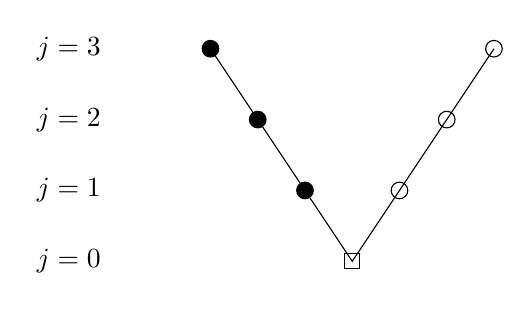
\begin{tikzpicture}[scale=1.2]
  \pgfmathsetmacro\hstep{0.5}
  \pgfmathsetmacro\vstep{0.75}
  \pgfmathsetmacro\ceps{0.08}   % size of square for coarse grid

% grid labels at left
  \node at (-2,3*\vstep) {$j=3$};
  \node at (-2,2*\vstep) {$j=2$};
  \node at (-2,\vstep) {$j=1$};
  \node at (-2,0.0) {$j=0$};

% V-cycle
  \draw[black,thin] (-\hstep,3*\vstep) -- (0.0,2*\vstep) -- (\hstep,\vstep) --  (2*\hstep,0.0)
                    -- (3*\hstep,\vstep) -- (4*\hstep,2*\vstep) -- (5*\hstep,3*\vstep);
  \filldraw (-\hstep,3*\vstep) circle (2.5pt);
  \filldraw (0.0,2*\vstep) circle (2.5pt);
  \filldraw (\hstep,\vstep) circle (2.5pt);
  \draw     (2*\hstep-\ceps,-\ceps) rectangle (2*\hstep+\ceps,+\ceps);
  \draw     (3*\hstep,\vstep) circle (2.5pt);
  \draw     (4*\hstep,2*\vstep) circle (2.5pt);
  \draw     (5*\hstep,3*\vstep) circle (2.5pt);
\end{tikzpicture}

\caption{A V-cycle on a three-level hierarchy ($K=2$) with a down-smoother (solid dots), up-smoother (circles), and coarse-level solver (square).}
\label{fig:vcycle}
\end{figure}

The above \textsc{vcycle} algorithm also calls a coarse solver on the $k=0$ level.  For a linear problem like our current Poisson problem it is traditional to apply a direct solver for this linear system (i.e.~equation \eqref{eq:linearsystem}), but this is not an option for the nonlinear glacier geometry problem.  Instead we suppose \textsc{coarsesolve} is implemented as a fixed number of GS sweeps.  If the coarsest mesh has a single node then a single sweep gives an exact solution.

We have now presented a basic geometric multigrid algorithm via a particular FE viewpoint, the subspace decomposition approach pioneered by Xu \cite{Xu1992} and others, an idea which applies both to multilevel and domain-decomposition algorithms.  We could now show computational results featuring the efficiency of the V-cycle algorithm, namely evidence of optimal $O(m_K)$ time to solve the problem.  (Such results appear in multigrid references \cite{Briggsetal2000,Bueler2021,Elmanetal2014,Trottenbergetal2001}.)  However, we first introduce a less-trivial ``obstacle'' problem which has the essential free-boundary character of the glacier geometry problem.  Computational results will be given in the next three sections.


\section{Multilevel constraint decomposition for the obstacle problem} \label{sec:obstacle}

\subsection*{An ice-like model problem}  We now have a basic view of the geometric multigrid (GMG) method from the multilevel subspace decomposition point of view.  However, as addressed in the Introduction, the main problem in glacier modeling, of how the ice geometry and velocity co-evolve in response to climatic inputs, needs an inequality constraint for well-posedness.  The fact that the ice surface elevation is above the bed generates the land-terminating boundary condition for the mass conservation problem, and this inequality constraint by itself makes the problem nonlinear.  It also reduces solution regularity in a manner which is challenging to numerical methods, with further challenges from the non-Newtonian viscosity of the fluid.

To address such inequality constraints, and before actually modeling glaciers in section \ref{sec:sia}, we introduce a more-convincing model problem, namely the \emph{classical obstacle problem}.  This simply adds an inequality constraint to the same linear differential equation, the Poisson equation.  After stating the weak form, which is now solved over a \emph{subset} of the function space, we will modify the multilevel subspace decomposition approach to be a \emph{constraint decomposition} method.  Each mesh level will host an inequality-constrained problem, and together all the levels will capture the original constraint set.  Switching the differential equation to the nonlinear SIA model in section \ref{sec:sia} will then be a comparatively easy change.

We use the same 1D domain and solution space $\mathcal{H}=H_0^1[0,1]$ as the Poisson problem \eqref{eq:poisson}.  Recall that functions in $\mathcal{H}$ have well-defined first derivatives and satisfy zero boundary conditions.  Let $\varphi(x)$ be a fixed function, also in $\mathcal{H}$, which is the obstacle.  The strong form of the obstacle problem is the following \emph{complementarity problem} (CP) \cite{Bueler2021,KinderlehrerStampacchia1980} which says that the Poisson equation applies whereever the solution $u(x)$ is strictly above the obstacle:
\begin{align}
  u - \varphi &\ge 0 \label{eq:obstaclecp} \\
  -u''-f &\ge 0 \notag \\
  (u-\varphi)(-u''-f) &= 0 \notag
\end{align}
The last condition, complementarity, implies that for each $x$ in $[0,1]$ the solution either coincides with the obstacle ($u(x)=\phi(x)$) or the Poisson equation holds at that point ($-u''(x)=f(x)$).  (Or both, but in the generic \emph{nondegenerate} \cite{KinderlehrerStampacchia1980} case the obstacle does not itself solve the Poisson equation.)  Conditions \eqref{eq:obstaclecp} also say that where the solution coincides with the obstacle the source term is bounded above: $u=\varphi \implies f \le -\varphi''$.  In this region, where $u=\varphi$, the constraint is said to be \emph{active}, while the (Poisson) differential equation holds in the \emph{inactive} portion where $u>\varphi$.

The glacier problem will also have a CP formulation (section \ref{sec:sia}; see also \cite{Calvoetal2002}).  The obstacle will be the bed elevation, the solution the glacier surface elevation, and the source term the surface mass balance.  In the inactive region, i.e.~on the glacier, the mass conservation equation will apply, but off the glacier, in the active region, the surface mass balance will be negative.

Simply by choosing a source term $f(x)$ which is positive in the middle of the domain and negative near the boundaries, we get an ``ice-like'' solution to \eqref{eq:obstaclecp} as shown in Figure \ref{fig:icelike}.  In detail, the Figure shows the exact, piecewise-quadratic solution $u(x)$ for the following data:
\begin{equation}
\varphi(x) = x(1-x) \quad \text{ and } \quad f(x) = \begin{cases} 8, & 0.2 < x < 0.8, \\
                                                               -16, & x<0.2 \text{ or } x>0.8. \end{cases}  \label{eq:icelikedetails}
\end{equation}
(Note that $f$ is in $L^2[0,1]$, and defined almost everywhere.)  Finding the formula for $u(x)$, which smoothly-connects five quadratic pieces, is an exercise for the reader.\footnote{Find the solution in: \, \href{https://github.com/bueler/mg-glaciers/blob/master/py/obstacle.py}{\texttt{github.com/bueler/mg-glaciers/blob/master/py/obstacle.py}}.}

% regenerate:
%   $ cd py/
%   $ ./obstacle.py -plain -kfine 5 -o icelike.pdf
%   $ pdfcrop icelike.pdf icelike.pdf
\begin{figure}
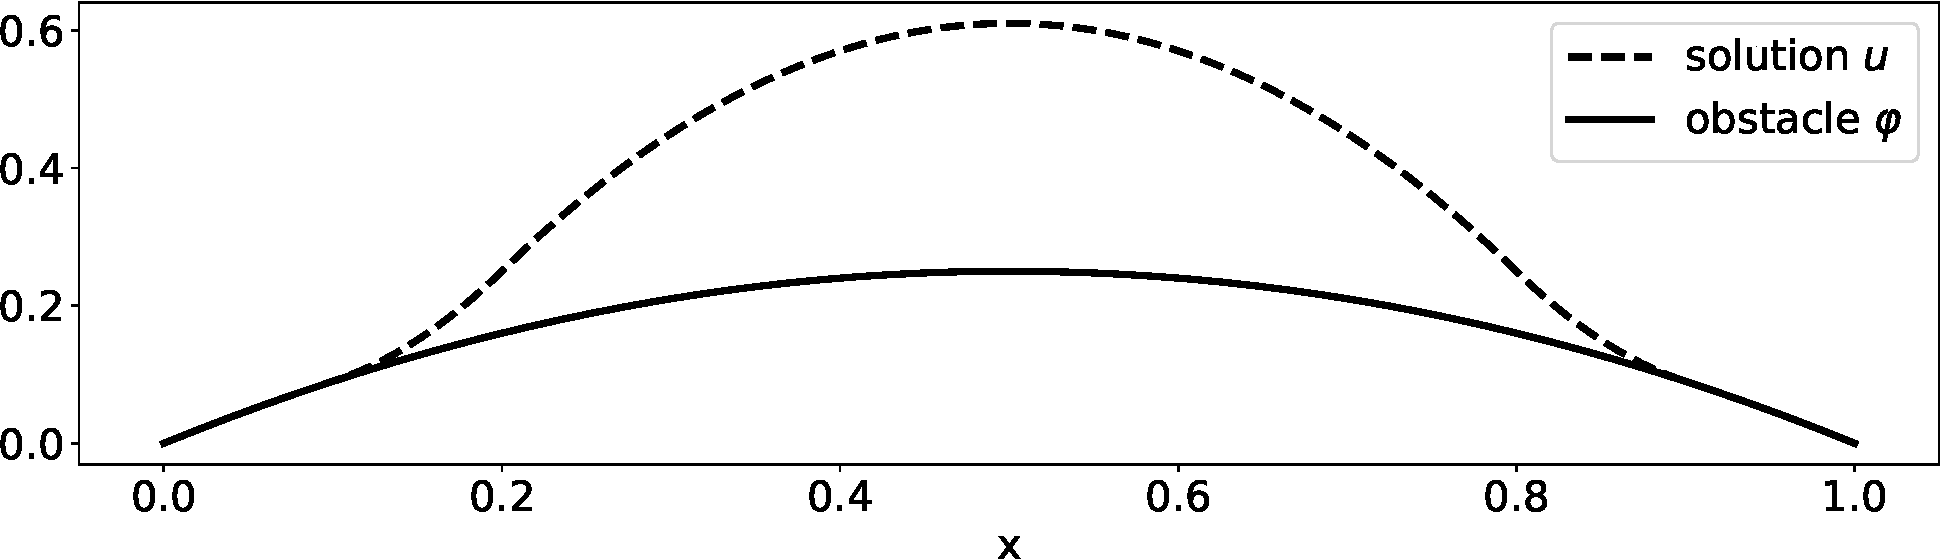
\includegraphics[width=0.7\textwidth]{fixfigs/icelike.pdf}
\caption{An ice-like configuration of the classical obstacle problem.}
\label{fig:icelike}
\end{figure}

Observe that the solution $u$ to \eqref{eq:obstaclecp} does not depend linearly on the source function $f$.  In fact, if $f(x)\le 0$ for all $x$ then the solution for the same obstacle $\varphi(x)=x(1-x)$ shown in Figure \ref{fig:icelike} is $u=\varphi$.  If $\tilde u$ solves the problem for $\tilde f= -1$, for example, then $2\tilde u$ \emph{does not} solve the problem for source term $2\tilde f = -2$.  In this sense the classical obstacle problem is nonlinear even though the corresponding PDE, the Poisson equation, which is the \emph{interior condition} of the CP \cite{KinderlehrerStampacchia1980}, is linear.

\subsection*{Weak formulation with constraints}  In considering the weak form of \eqref{eq:obstaclecp} we observe that the solution and test functions must be in a closed subset which incorporates the constraint:
\begin{equation}
\mathcal{K} = \left\{v \ge \varphi\right\} \subseteq \mathcal{H}.  \label{eq:Kdefine}
\end{equation}
This subset is not a vector space, but it is \emph{convex}.  That is, if $v,w$ are in $\mathcal{K}$ then any point on the line segment connecting them, namely $\alpha v + (1-\alpha) w$ for $0 \le \alpha \le 1$, is also in $\mathcal{K}$.  

As expected, derivation of the weak form of \eqref{eq:obstaclecp} involves multiplying by a test function and integrating by parts.  However, the inequalities enter nontrivially into the derivation; see \cite[Chapter 12]{Bueler2021}, \cite{JouvetBueler2012}, or \cite{KinderlehrerStampacchia1980}.  The result is a single \emph{variational inequality} (VI):
\begin{equation}
  a(u,v-u) \ge \ip{f}{v-u} \quad \text{ for all } v \text{ in } \mathcal{K}. \label{eq:obstaclevi}
\end{equation}
The bilinear form on the left is the same as in equation \eqref{eq:weakpoisson}: $a(u,v) = \int_0^1 u'(x) v'(x)\,dx$.

Inequality problems \eqref{eq:obstaclecp} and \eqref{eq:obstaclevi} are equivalent up to the same regularity concerns which relate the strong and weak forms of a PDE.  (See reference \cite{Evans2010} regarding the solution regularity of PDEs, and \cite{KinderlehrerStampacchia1980} for the corresponding VI concepts.)  However, the intuition behind a VI is needed for understanding.  To help, we provide another weak form.  Inequality \eqref{eq:obstaclevi} is precisely equivalent to \emph{constrained minimization}:
\newcommand{\argmin}{\mathop{\mathrm{arg\text{-}min}}}
\begin{equation}
  u = \argmin_{w \text{ in } \mathcal{K}} J(w) \quad \text{where} \quad J(w) = \frac{1}{2} a(w,w) - \ip{f}{w}. \label{eq:obstaclemin}
\end{equation}
That is, $u$ is the minimizer, over the constraint set $\mathcal{K}$, of the scalar, quadratic \emph{objective} functional $J$.  The proof of equivalence is standard in continuous optimization.  One computes the (Gateaux) derivative, a linear functional in $\mathcal{H}'$:
\begin{equation}
  \grad J(w)[v] = \lim_{\eps\to 0} \frac{J(w+\eps v) - J(w)}{\eps} = a(u,v) - \ip{f}{v}.  \label{eq:gradobjective}
\end{equation}
This gradient $\nabla J(u)$ already appears in \eqref{eq:obstaclevi}, and the VI can be re-stated as follows:
\begin{equation}
  \nabla J(u)[v-u] \ge 0 \quad \text{ for all } v \text{ in } \mathcal{K}. \label{eq:obstaclevigradient}
\end{equation}

The solution $u$ of \eqref{eq:obstaclevi}, \eqref{eq:obstaclemin}, or \eqref{eq:obstaclevigradient} sits at a location in $\mathcal{K}$, possibly on the boundary of $\mathcal{K}$, where a vector pointing further into the constraint set, namely $v-u$ for $v$ in $\mathcal{K}$, points ``uphill'' on the graph of $J$.  If we think of $\nabla J(u)$ as a vector, instead of a linear functional, we could write \eqref{eq:obstaclevigradient} as $\ip{\nabla J(u)}{v-u} \ge 0$, thus the angle between $\nabla J(u)$ and $v-u$ is at most 90 degrees.  One possibility for our 1D obstacle problem is that the constraint is strict for every $x$, i.e.~$u(x) > \varphi(x)$, in which case \eqref{eq:obstaclevigradient} implies the unconstrained minimum condition $\nabla J(u)[v] = 0$ for all $v$ in $\mathcal{H}$; in this case the gradient of $J$ is zero at $u$.

Of course, $\mathcal{K}$ in \eqref{eq:Kdefine} is an infinite-dimensional set.  To aid the intuition we propose the following low-dimensional, but global, mental image.  Imagine the constraint set $\mathcal{K}$ as analogous to the closed first quadrant in the plane, $\mathcal{Q} = \left\{(x_1,x_2)\,:\,x_i\ge 0\right\}$, and $J$ as analogous to a smooth, concave-up (i.e.~\emph{coercive} \cite{Evans2010}), objective function $\gamma(x_1,x_2)$ defined on the plane.  The solution of the corresponding VI, say $(\hat x_1,\hat x_2)$ in $\mathcal{Q}$, may not be a location where $\nabla \gamma$ is zero.  However, it will have as low a value of $\gamma$ as possible, even if it is on the boundary of $\mathcal{Q}$.  At $(\hat x_1,\hat x_2)$ all directions \emph{into} $\mathcal{Q}$ will increase the value of $\gamma$, as sketched by contours in Figure \ref{fig:cartoonplane}.  The obstacle problem solution shown in Figure \ref{fig:icelike} is an infinite-dimensional version of the solution point shown in the Figure \ref{fig:cartoonplane} cartoon view.

\begin{figure}
\includegraphics[width=0.35\textwidth]{genfigs/cartoonplane.pdf}
\caption{For analogy only:  A 2-dimensional constrained-minimization or VI solution, in a planar quadrant $\mathcal{Q}$, with contours of a scalar function $\gamma(x_1,x_2)$.}
\label{fig:cartoonplane}
\end{figure}

The glacier problem in the next section will also be formulated as a CP like \eqref{eq:obstaclecp}, and as a VI like \eqref{eq:obstaclevi}.  However, for general bed elevation functions (obstacles) the glacier problem has no constrained minimization formulation like \eqref{eq:obstaclemin}; the essential reason is the lack of symmetry of the weak form in the general case \cite{JouvetBueler2012}.  In other words, for the glacier problem we possess a map like $\grad J$, from $\mathcal{H}$ to $\mathcal{H}'$, but not a scalar objective like $J$ itself.  We will return to this point in section \ref{sec:sia}.

Regardless of how the classical obstacle problem is formulated, a \emph{free boundary} generally arises in the interior of the domain.  For example, as we move away from the midpoint in Figure \ref{fig:icelike} there are locations, near the ends of $[0,1]$, where the solution first becomes fully in contact with the obstacle.  At these locations both $u=\varphi$ and $u'=\varphi'$ hold, that is, the solution is tangent to the obstacle at the free boundary.  These simultaneous Dirichlet and Neumann ``conditions'' occur at a location which must be found as part of the solution.  (In addition, there are fixed boundary conditions because the solution $u$ is in $\mathcal{H}$.)

The solution of the classical obstacle problem can be non-smooth at the free boundary even when the data is arbitrarily smooth.  For example, smoothing the source term $f$ in \eqref{eq:icelikedetails} would give a solution nearly the same as shown in Figure \ref{fig:icelike}.  That is, one could make the source term $f$ into a smooth function by ``mollification'' \cite{Evans2010} so that the transition between positive and negative values of $f$ would be $C^\infty$.  However, the free boundary would remain, and at that free boundary the second derivative $u''$ would jump from value $+16=-f$ to value $-2=\varphi''$.  Thus the 1D obstacle problem solution, for smooth data, is limited to the Sobolev space $W^{2,\infty}$ \cite[section IV.6]{KinderlehrerStampacchia1980}, and (generally) not smoother.

\subsection*{Constraint decomposition}  Recall from section \ref{sec:subspace} that each mesh level corresponds to $m_k$ hat functions $\psi_p^k(x)$, at interior nodes $x_p^k$, and to the corresponding vector space $\mathcal{V}_k$ of piecewise-linear functions with value zero at $x=0,1$.  (See Figures \ref{fig:finehats}, \ref{fig:coarsehats}.)  In this section we add an obstacle function $\phi^k(x)$ on each level, to define a closed, convex $k$\emph{th-level constraint set}
\begin{equation}
\mathcal{K}^k = \left\{v \text{ in } \mathcal{V}^k \text{ such that } v \ge \phi^k\right\}.  \label{eq:levelKdefine}
\end{equation}
However, the construction of the $k$th-level obstacle $\phi^k$ is nontrivial; it is \emph{not} the $k$th-level interpolant of the continuum obstacle $\varphi$.  Indeed, the manner in which we decompose the continuum constraint $\mathcal{K}$ into multilevel sets $\mathcal{K}^k$ is the key concern of this section.  On the $k$th level we have the finite-dimensional VI for $u^k$ in $\mathcal{K}^k$:
\begin{equation}
  a(u^k,v-u^k) \ge \ell^k[v-u] \quad \text{ for all } v \text{ in } \mathcal{K}^k. \label{eq:levelvi}
\end{equation}
As in the previous section, $\ell^K[v]=\ip{f}{v}$ on the finest level, but on coarser levels we will redefine the linear functional $\ell^k$ for the right-hand side.

As we did for GMG on the Poisson equation, on each mesh level we can immediately propose an iterative solution method for the weak form \eqref{eq:levelvi}.  The \emph{projected Gauss-Seidel (PGS) iteration} is a small modification of the original GS method.  This method might ultimately solve the problem---a proof is in \cite{BrandtCryer1983}---but here it serves as a smoother; we only apply one or two iterations on each level.  The PGS iteration finds the solution to VI \eqref{eq:levelvi}, though slowly, by approximately descending the gradient $\grad J$ while remaining in the constraint region $\mathcal{K}^k = \{w\ge \phi^k\}$.  Specifically, PGS descends by adjusting the iterate one point at a time.  Recall that conventional GS successively zeros the residual at points, i.e.~it finds $c$ so that $r^k(w+c\psi_p^k)[\psi_p^k]=0$, but the residual is the same as the \emph{negative} gradient of the objective:
\begin{equation}
  r^k(w)[v] = - \grad J^k(w)[v].  \label{eq:levelresidualgradient}
\end{equation}
Also, because $\mathcal{K}^k$ consists of piecewise-linear functions, if $w$ is in $\mathcal{K}^k$ then one can test whether the modified iterate is still in $\mathcal{K}^k$ via a pointwise comparison, i.e.~testing $w[p] + c \ge \phi^k[p]$.  Thus we have the following smoother algorithm:
\begin{pseudo*}
\pr{pgssweep}(k,w,\ell,\phi)\text{:} \\+
    for $p=1,\dots,m_k$ \\+
        $\displaystyle c = r^k(w)[\psi_p^k] \, \big/ \,a(\psi_p^k,\psi_p^k)$ \qquad \ct{where $r^k(w)[\cdot] := \ell[\cdot] - a(w,\cdot)$} \\
        $w[p] \gets \max\{w[p] + c,\phi[p]\}$
\end{pseudo*}

However, we still need to define the $k$th-level obstacle $\phi^k$.  Suppose that on the fine level we have a solution method which computes iterates $w^K$ in $\mathcal{K}^K$ which converge to the solution $u^K$ of the fine level problem \eqref{eq:levelvi}.  (Applying PGS on the fine level would generate such iterates, but they would converge very slowly.)  Define $\varphi^K$ to be the piecewise-linear interpolant (i.e.~in $\mathcal{V}^K$) of the continuum obstacle $\varphi$.  We define the \emph{defect constraint} \cite{GraeserKornhuber2009} on the fine level to be
\begin{equation}
  \chi^K = \varphi^K - w^K.  \label{eq:defectconstraint}
\end{equation}
Note that admissibility for the iterate $w^K$ is equivalent to a nonpositive defect constraint: $w^K \ge \varphi^K \iff 0 \ge \chi^K$.  More generally, if we modify an iterate $w^K$ by adding $v$ then the result is admissible if and only if $v$ is above the defect constraint:
\begin{equation}
  w^K + v \ge \varphi^K  \qquad \iff \qquad v \ge \chi^K.  \label{eq:defectmeaning}
\end{equation}
This is the essential meaning of ``defect constraint.''

A main principle for our constraint decomposition method is that
\begin{quote}
\emph{as much as possible of the fine-level defect constraint $\chi^K$ is in the coarsest levels.}
\end{quote}
We will define coarser-level versions of the defect constraint, namely $\chi^k$ in equation \eqref{eq:chik} below, for all levels $k=0,1,\dots,K-1$.  From these we define the \emph{$k$th-level obstacles}:
\begin{equation}
  \phi^k = \chi^k - P\chi^{k-1} \quad \text{ for } k=1,2,\dots,K, \text{ and } \quad \phi^0 = \chi^0.  \label{eq:levelobstacle}
\end{equation}
Recall from section \ref{sec:subspace} that the canonical prolongation operator $P$ actually does nothing; in definition \eqref{eq:levelobstacle} it takes $\chi^{k-1}$ in $\mathcal{V}^{k-1}$ to the same function $P\chi^{k-1}$ in $\mathcal{V}^k$.  Therefore, from now on we simply write $\phi^k = \chi^k - \chi^{k-1}$.

The multilevel constraint decomposition is now a ``telescoping'' sum:
\begin{equation}
  \sum_{k=0}^K \phi^k = \chi^0 + (\chi^1 - \chi^0) + (\chi^2 - \chi^1) + \dots + (\chi^K - \chi^{K-1}) = \chi^K.  \label{eq:telescopingdecomposition}
\end{equation}
That is, we have decomposed the fine-level defect constraint $\chi^K$ into the obstacles $\phi^k$ which we will actually use on each level.  (Note that the sum does \emph{not} give a decomposition of the original obstacle $\varphi$, and it depends on a fine-mesh iterate.)  An example decomposition is shown in Figure \ref{fig:gooddecomposition}; compare Figure 1 in \cite{GraeserKornhuber2009}.

%REGENERATE Figures \ref{fig:icelikedecomposition} and \ref{fig:gooddecomposition}:
%$ ./obstacle.py -kfine 5 -irtol 1.0e-7 -random -randommodes 8 -diagnostics -up 0 -o defect.pdf
%fine level 5 (m=63) using 52 V(1,0) cycles (102.375 WU)
%saving final iterate and obstacle to defect.pdf ...
%saving residual and inactive residual to resid_defect.pdf ...
%saving hierarchical decomposition to decomp_defect.pdf ...
%saving "ice-like" decomposition to icedec_defect.pdf ...
\begin{figure}
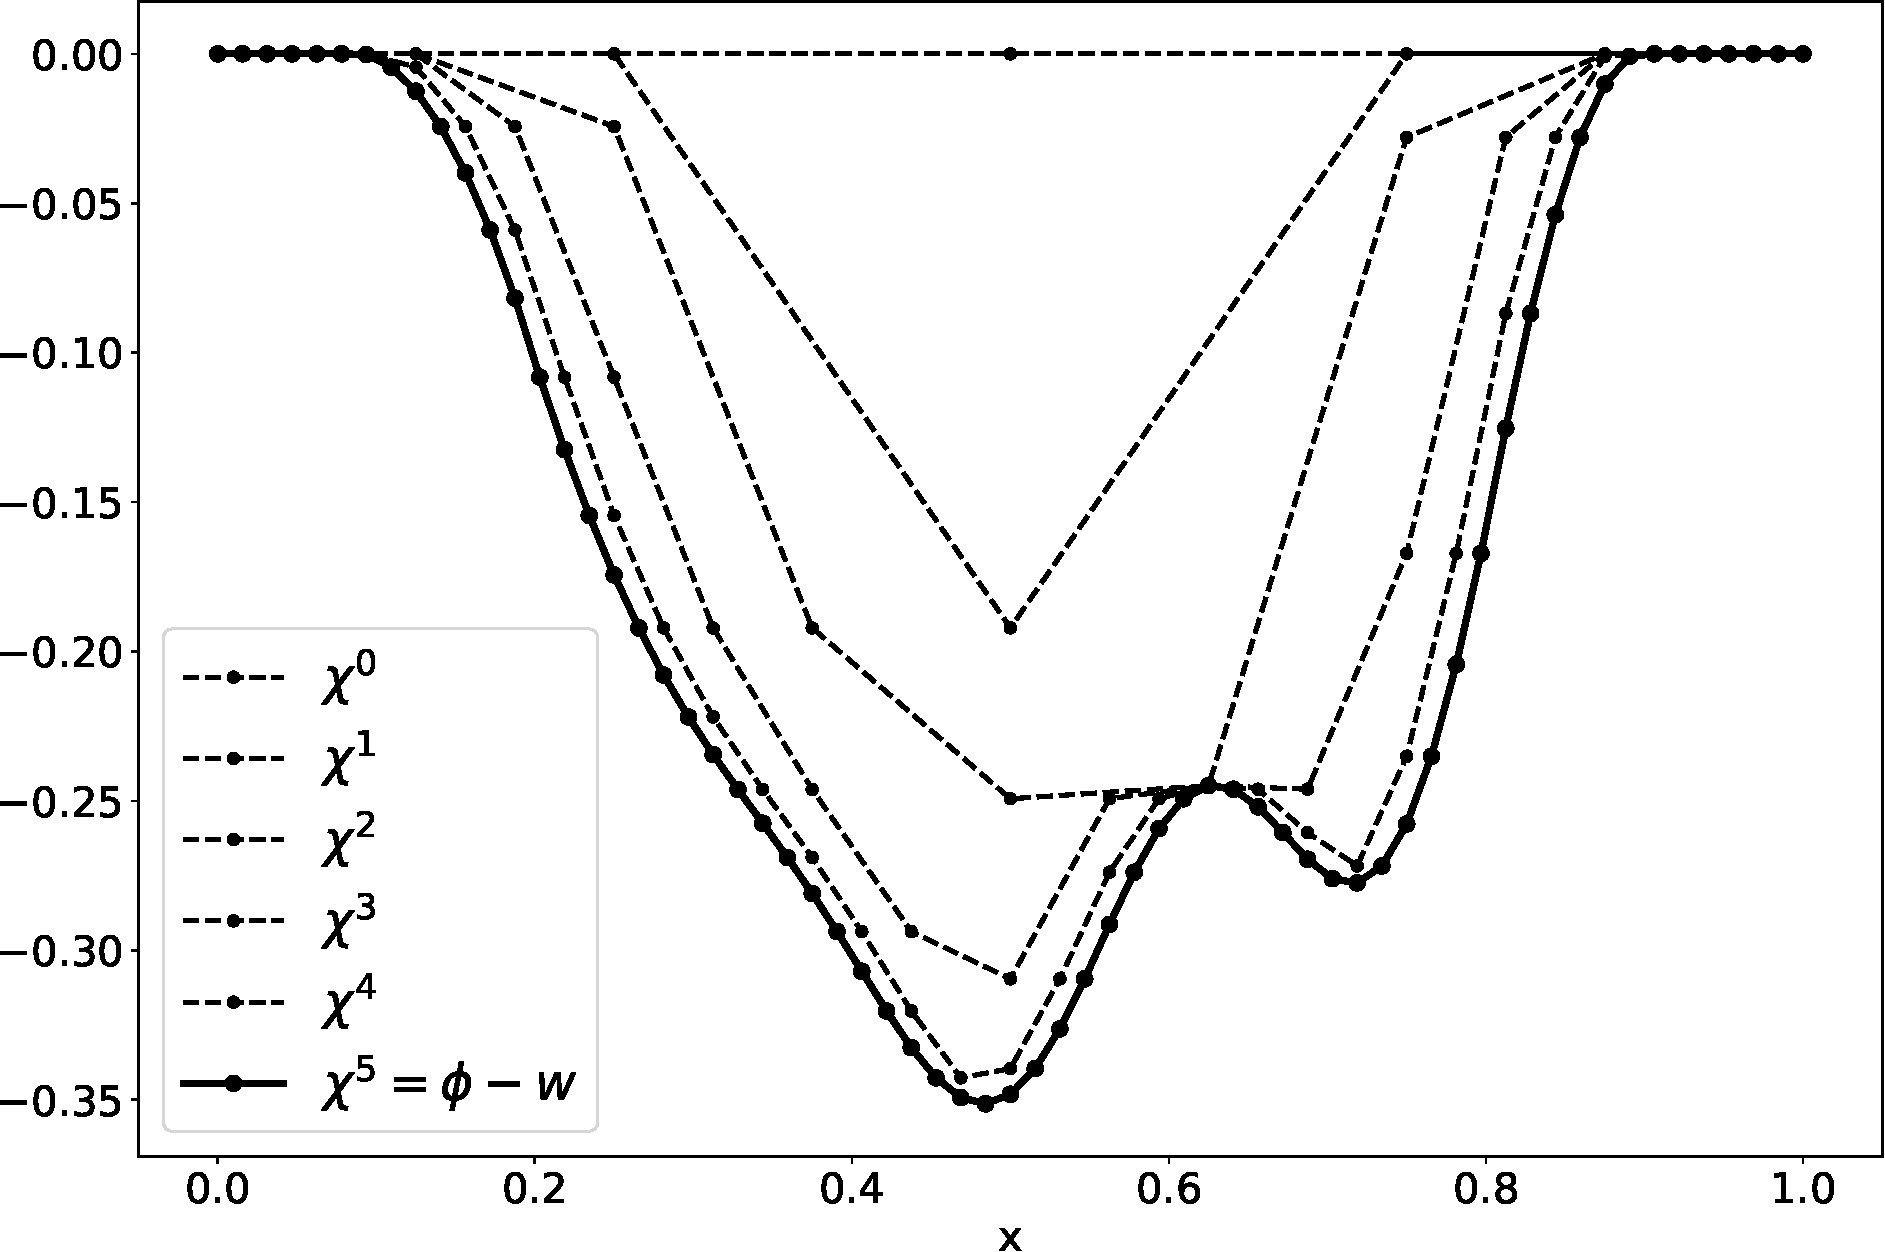
\includegraphics[width=0.75\textwidth]{fixfigs/decomp_defect.pdf}
\caption{The constraint decomposition writes the fine-mesh defect obstacle $\chi^K = \varphi^K - w^K$ as a sum of the obstacles (gaps) $\phi^k = \chi^k - \chi^{k-1}$ on each level.  The $k$th-level constraint set in our multilevel method is $\mathcal{K}^k = \{v \ge \phi^k\} \subseteq \mathcal{V}^k$.}
\label{fig:gooddecomposition}
\end{figure}

However, we need to define the coarser-level defect constraints $\chi^k$.  On the fine level we have already set $\chi^K = \varphi^K - w^K$, and we now define the others inductively, down to the coarsest mesh ($k=0$), so that each difference $\phi^k = \chi^k - \chi^{k-1}$ is nonpositive (Figure \ref{fig:gooddecomposition}).  That is, our goals are that $\chi^{k-1}$ is in $\mathcal{V}^{k-1}$ and that $\chi^{k-1}(x) \ge \chi^k(x)$ for all $x$ in $[0,1]$.  Thus we define a \emph{monotone restriction} operator $\hat R$ from $\mathcal{V}^k$ to $\mathcal{V}^{k-1}$.  For $z$ in $\mathcal{V}^k$ one computes $\hat R z$ by maximizing the node values of $z$ over the interior of the support of each level $k-1$ hat function.  That is, if $z = \sum_{q=1}^{m_k} b_q \psi_q^k$ then
\begin{equation}
  \hat R z = \sum_{p=1}^{m_{k-1}} c_p \psi_p^{k-1} \qquad \text{where} \qquad c_p = \max_{\psi_p^{k-1}(x_q^k) > 0} b_q.  \label{eq:monotonerestriction}
\end{equation}
Recall that our hat functions form nodal bases, and thus $c_p = (\hat R z)(x_p^{k-1})$, for example.  Also note that while canonical restriction \eqref{eq:canonicalrestriction} acts on linear functionals ($(\mathcal{V}^k)'$), monotone restriction acts on functions ($\mathcal{V}^k$).  Finally define
\begin{equation}
  \chi^{k-1} = \hat R \chi^k.  \label{eq:chik}
\end{equation}

Each $k$th-level obstacle $\phi^k = \chi^k - \chi^{k-1}$ also defines a constraint set
\begin{equation}
  \mathcal{K}^k = \{v \ge \phi^k\} \subseteq \mathcal{V}^k.  \label{eq:levelconstraint}
\end{equation}
Given a fine-mesh iterate $w^K$ and the corresponding defect constraint $\chi^K = \varphi^K - w^K$, we have a sum of subsets which is analogous to \eqref{eq:subspacedecomposition}:
\begin{equation}
  \left\{v\,:\,w^K + v \ge \varphi^K\right\} = \left\{v \ge \chi^K\right\} = \mathcal{K}^0 + \mathcal{K}^1 + \dots + \mathcal{K}^K. \label{eq:constraintdecomposition}
\end{equation}
The meaning here is that every admissible modification $v$ of the current fine-mesh iterate---by \eqref{eq:defectmeaning} this is every $v$ above the fine-mesh defect constraint $\chi^K$---can be built, though not uniquely, by choosing an element from each of the mesh-level constraint sets $\mathcal{K}^k = \{v \ge \phi^k\}$.  Note that the proof of \eqref{eq:constraintdecomposition} is an inequality version of the telescoping sum \eqref{eq:telescopingdecomposition}.

In the ice context (section \ref{sec:sia}) the fine-mesh obstacle $\varphi^K$ will be the bed elevation and $w^K$ a current estimate of the ice surface elevation.  Thus $-\chi^K$ is the ice thickness on the fine mesh.  Figure \ref{fig:icelikedecomposition} shows the same constraint decomposition as in Figure \ref{fig:gooddecomposition} as though it is a decomposition of the ice into layers.  (Compared to Figure \ref{fig:icelike}, note that this bed elevation $\phi^K$ has a more interesting, but still smooth, bed topography.)  However, Figure \ref{fig:gooddecomposition} plots the decomposition in the correct sense: each defect constraint $\chi^k$ and obstacle $\phi^k$ is piecewise-linear on level $k$.

\begin{figure}
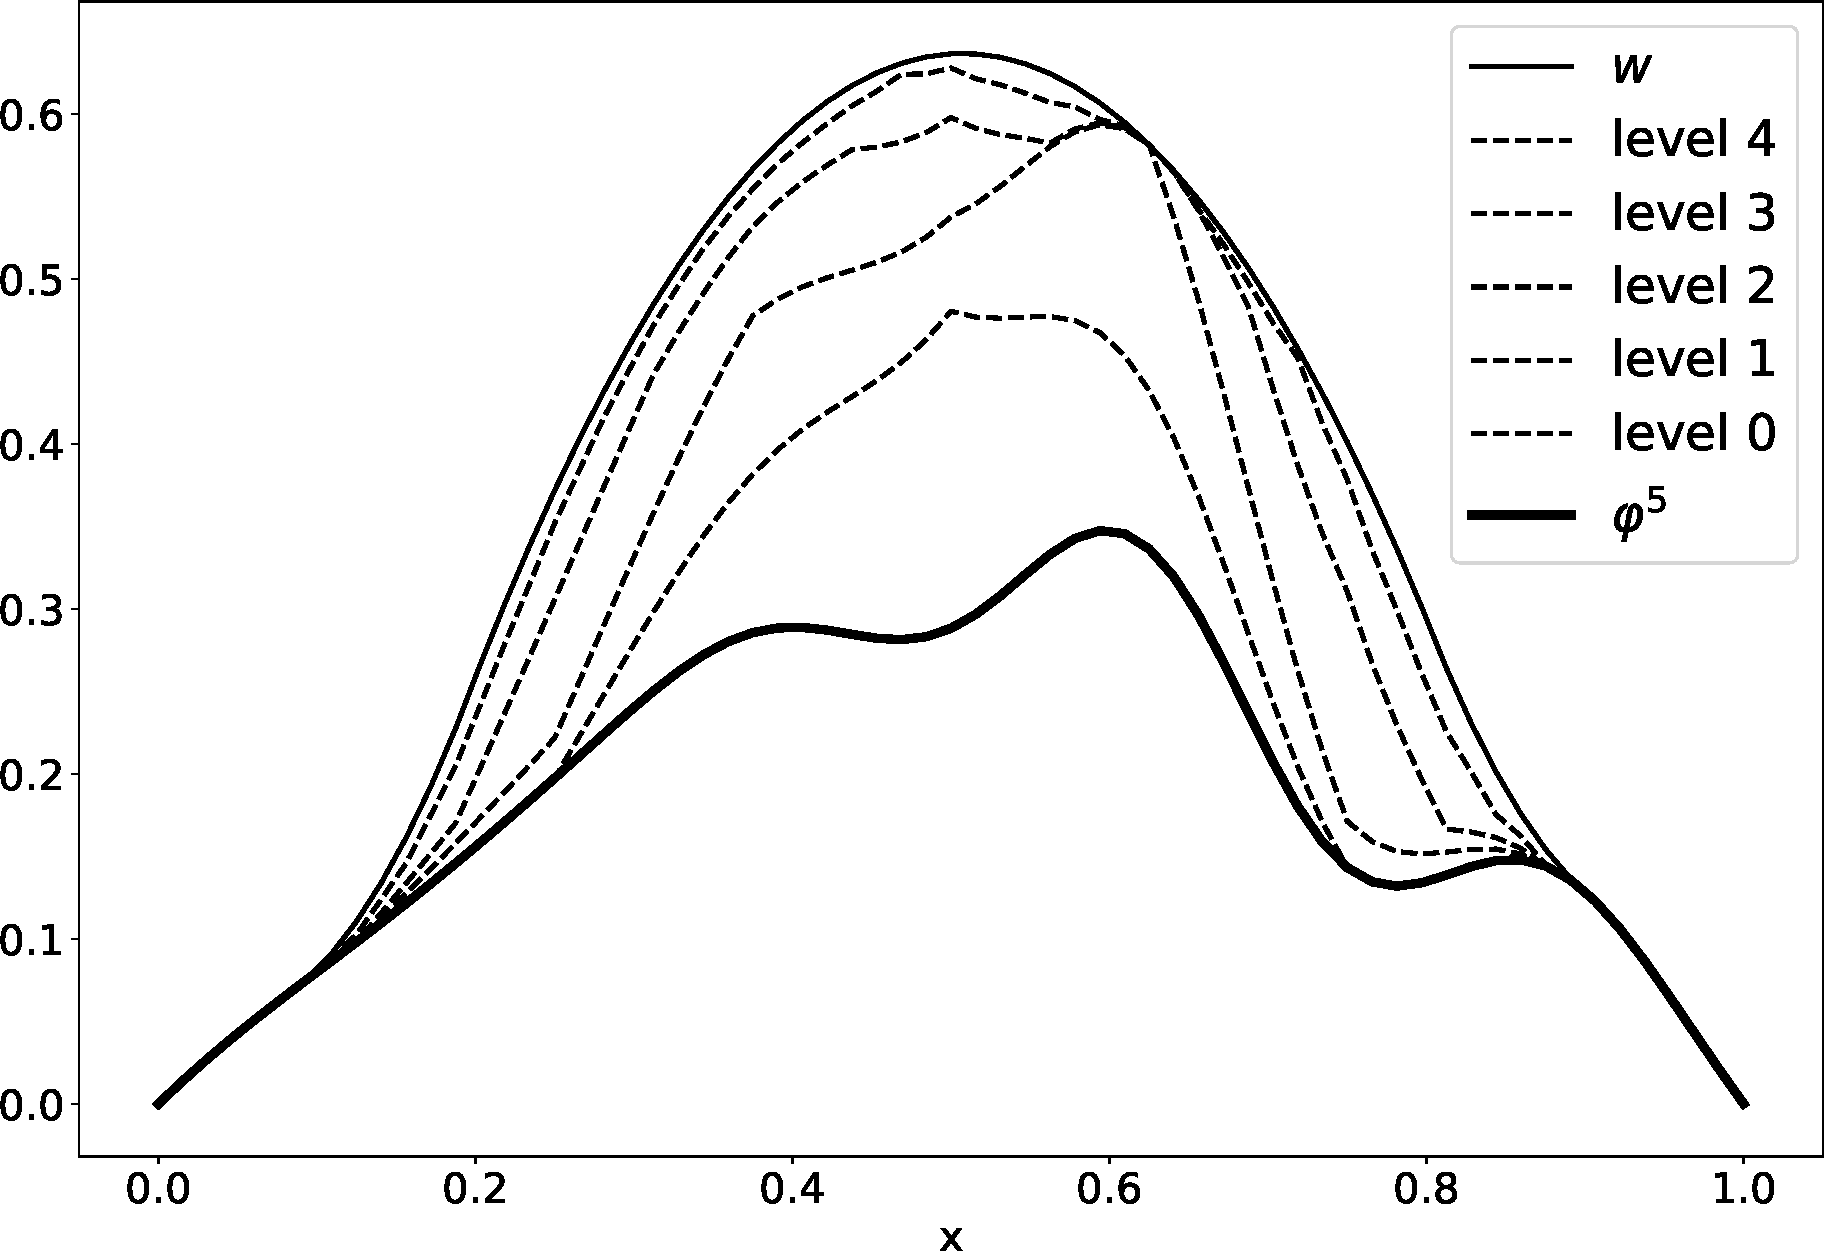
\includegraphics[width=0.7\textwidth]{fixfigs/icedec_defect.pdf}
\caption{The multilevel constraint decomposition, visualized as a decomposition of the ``ice'' between the current fine-mesh iterate $w$ and the obstacle $\varphi^K$.  (Figure \ref{fig:gooddecomposition} shows the correct plot of this constraint decomposition.)}
\label{fig:icelikedecomposition}
\end{figure}

FIXME state V-cycle for V(1,0); run as \pr{cd-slash}$(K,r^K,\chi^K)$ where $w^K$ is an existing admissible fine-mesh iterate, $\chi^K=\varphi^K-w^K$, and $r^K[\cdot] = \ell^K[\cdot] - a(w^K,\cdot)$; use the result $v$ to update the iterate: $w^K \gets w^K + v$
\begin{pseudo*}
\pr{cd-slash}(k,r,\chi)\text{:} \\+
    $v=0$ \\
    if $k=0$ \\+
        $\text{\pr{pgssweep}}^{\text{\id{coarse}}}(0,v,r,\chi)$ \\
        return $v$ \\-
    $\chi^{k-1} = \hat R \chi$ \\
    $\phi^k = \chi - P\chi^{k-1}$ \\
    $\text{\pr{pgssweep}}^{\text{\id{down}}}(k,v,r,\phi^k)$ \\
    $\tilde r[\cdot] = r[\cdot] - a^k(v,\cdot)$ \\
    $v^{k-1} =$ \pr{cd-slash}(k-1,R \tilde r,\chi^{k-1}) \\
    return $v + P v^{k-1}$
\end{pseudo*}


FIXME state V(1,1)-cycle; run the same way
\begin{pseudo*}
\pr{cd-vcycle}(k,r,\chi)\text{:} \\+
    $v=0$ \\
    if $k=0$ \\+
        $\text{\pr{pgssweep}}^{\text{\id{coarse}}}(0,v,r,\chi)$ \\
        return $v$ \\-
    $\chi^{k-1} = \hat R \chi$ \\
    $\phi^k = \frac{1}{2} (\chi - P\chi^{k-1})$ \\
    $\text{\pr{pgssweep}}^{\text{\id{down}}}(k,v,r,\phi^k)$ \\
    $\tilde r[\cdot] = r[\cdot] - a^k(v,\cdot)$ \\
    $v^{k-1} =$ \pr{cd-vcycle}(k-1,R \tilde r,\chi^{k-1}) \\
    $v \gets v + P v^{k-1}$ \\
    $\text{\pr{pgssweep}}^{\text{\id{up}}}(k,\hat v,r,\phi^k)$ \\
    return $v$
\end{pseudo*}

FIXME cite for multigrid obstacle \cite{BrandtCryer1983,Bueler2021,GraeserKornhuber2009,Jouvetetal2013}; cite for subset decomp \cite{Tai2003}

\subsection*{Results} FIXME


\section{Multigrid for a shallow-ice mass conservation problem} \label{sec:sia}

FIXME model problem in previous section has the wrong ``physics'' but correctly addresses the free boundary and obstacle nature of the glacier problem

FIXME cite for glaciers as obstacle problems \cite{Bueler2016,Bueler2020,Calvoetal2002,JouvetBueler2012}

FIXME for 2D domains the coarse mesh construction needs reconsideration


\section{Multigrid for a Glen-Stokes glacier flow} \label{sec:stokes}

FIXME multigrid already used for Blatter-Pattyn model \cite{BrownSmithAhmadia2013} and for hybrid \cite{Jouvetetal2013}; one goal of this section is to make these approaches more understandable

FIXME we use Schur complement \cite{Bueler2021,Elmanetal2014} and compare it to Vanka monolithic smoother \cite{Farrelletal2019}

\small

\bigskip
\bibliography{review}
\bibliographystyle{siam}

\normalsize
%\clearpage

\appendix
\section{Notation}

\renewcommand{\arraystretch}{1.2}
\begin{longtable}{l|l}
\textbf{Symbol} {\Large$\strut$} & \textbf{Meaning} \\ \hline
$a(\cdot,\cdot)$ & bilinear form associated to the Poisson problem; left side of equation \eqref{eq:weakpoissonearly} \\
$\mathcal{H}$ & Hilbert space for the continuum problem \\
$J$ & scalar-valued objective function, e.g.~$J(v) = \frac{1}{2} a(v,v) - \ip{f}{v}$ for the Poisson equation \\
$\grad J(w)[v]$ & gradient of objective function; note $r(w)[v] = -\grad J(w)[v]$ \\
$k$ & index of level in multilevel scheme; $k=0,1,\dots,K$ from coarse to fine \\
$\mathcal{K}$ & constraint (admissible) subset; $\mathcal{K} \subset \mathcal{H}$; e.g.~$\mathcal{K} = \{v \ge \phi\}$ \\
$\mathcal{K}^k$ & $k$th-level admissible functions; $\mathcal{K}^k = \{v \ge \phi^k\} \subset \mathcal{V}^k$ \\
$\ell[\cdot]$ & linear functional, e.g.~$\ell[v] = \ip{f}{v}$ \\
$m_k$ & number of nodes in $k$th-level; $\dim \mathcal{V}^k=m_k$ \\
$P$ & canonical prolongation of functions; equation \eqref{eq:canonicalprolongation} \\
$R$ & canonical restriction of linear functionals; equation \eqref{eq:canonicalrestriction} \\
$\hat R$ & monotone restriction of functions; equation \eqref{eq:monotonerestriction} \\
$r(w)[\cdot]$ & residual of iterate $w$, e.g.~$r(w)[v] = \ip{f}{v} - a(w,v)$ for the Poisson equation \\
$\mathcal{V}^h$ & finite element function space; $= \mathcal{V}^K$ \\
$\mathcal{V}^k$ & $k$th-level vector space \\
$(\mathcal{V}^k)'$ & dual of $k$th-level vector space ($=$ linear functionals) \\
$x_p^k$ & $p$th node on $k$th-level mesh \\
$\varphi$ & obstacle in continuum problem \\
$\phi^k(x)$ & $k$th-level obstacle in constraint decomposition method; $\phi^k=\chi^k - P\chi^{k-1}$ \\
$\psi_p^k(x)$ & $k$th-level hat function at $x_p$ \\
$\chi^k(x)$ & $k$th-level (monotone) restriction of defect obstacle; $\chi^K = \varphi^K - w^K$ and $\chi^{k-1} = \hat R \chi^k$ \\
$\ip{\cdot}{\cdot}$ & $L^2$ inner product \\
$\|\cdot\|$ & $L^2$ norm; $\|f\|=\ip{f}{f}^{1/2}$
\end{longtable}

\end{document}
